I will introduce a preliminary definition of the Berkovich spectrum of a ring, which for now will just be a topological space. 
It will serve to build intuition for Berkovich spaces by exploring the Berkovich spectrum of two rings $\Z$ and $K[T]$ where $K$ is a complete algebraically closed field, with non-trivial absolute value. 

\begin{definition}
	Let $A$ be a ring. We define \[
		\mathcal{M} (A) = \{x: A \to \R^{+} \st \text{multiplicative seminorm on } A\} 
	.\] 
	This comes equipped with the coarsest topology such that for every $f \in A$ the map $\mathcal{M} (A) \to [0, \infty) : \|\cdot \|_x \mapsto \|f\|_x $ is continuous. 

	We will almost always deal with a relative case where $A$ is a $k$-algebra over some real valued field $K$. In this case adjust the definition \[
		\mathcal{M} (A) = \{x : A \to \R^{ + }  \mid \text{multiplicative seminorm on }A \text{ extending the norm on } K\} 
	.\] 
	Again $\mathcal{M} (A)$ comes with the coarsest topology making all maps $\mathcal{M} (A) \to [0, \infty): x \mapsto \|f\|_x, \forall f \in A$ continuous. 
\end{definition}
We think of $\mathcal{M} (A)$ as a geometric space and thus its elements are points, usually denoted by a letter, like $x$. 
For an element $f \in A$ we write $|f|_x$ or $x(f)$ for  $f$ evaluated in the norm $x$. 

\begin{remark}
	$\mathcal{M}$ is not only a map, but it is also a contravariant functor. 
	Let $A, B$ be two rings and $f: A \to B$ a morphism. 
	Then a seminorm $x \in \mathcal{M} (B)$ turns into a seminorm on $\mathcal{M} (A)$ by defining $\mathcal{M} (f)(x): A \to \R^{ +}: a \mapsto |f(a)|_x$.


This is analogous to the $\spec$ functor and there even is a natural transformation $\mathcal{M} \implies \spec$ defined by $\mathcal{M} (A) \to \spec A: |\cdot |_x \mapsto \ker x$. This is well defined by \cref{rem:ker_norm_ideal}. 
\end{remark}

There also is a generalisation of the residue field at a prime ideal. 

\begin{definition}\label{def:completed_residue_field}
	Let $A$ be a ring (possibly over $K$) and $x \in \mathcal{M} (A)$ a point in its Berkovich spectrum. 
	Then the \emph{completed residue field at $x$} is defined as \[
		\mathcal{H} (x) = (Q(A / \ker x), |\cdot |_x)^{\wedge}
	.\] 
	This is the completion of $A / \ker x$ with respect to the norm induced by $x$. 
	It comes with a induced morphism $\chi_x: A \to \mathcal{H} (x)$.
	\question{its not really necessary to take the kernel here right? Completing will already do that because they will be equivalent cauchysequences?}
\end{definition}

Like $\spec$, the points in $\mathcal{M} $ can be described as \emph{characters}, i.e.  maps $\chi: A \to L$ (over $K$) where $L$ is a complete valued field subject to the condition that $\chi_1: A \to L_1, \chi_2: A \to L_2$ are equivalent if there exists another map to a complete valued field $\chi: A \to L$  and maps $L \to L_1, L \to L_2$ extending the norm on $L$ such that the diagram 
\[
\begin{tikzcd}
	& A \ar{dl}[']{\chi_1} \ar{dr}{\chi_2} \dar{\chi} \\
	L_1 & L \lar \rar & L_2
\end{tikzcd}
\] 
commutes. 
For any point $x$ the map $\chi_x: A \to \mathcal{H} (x)$ gives a minimal representative for the character corresponding to the point $x$. 


\begin{remark}
	Later we will consider other topologies on $X\an$, which will be necessary to turn $X\an $ into a ringed space. 
	There topologies will not be topologies like we know it. They will be Grothendieck topologies, where which unlike ordinary topologies restrict the notion of a cover. 
\end{remark}

\begin{proposition}\label{prop:spec_ring_haussdorf}
	Let $R$ be a ring then $\mathcal{M} (R)$ is Hausdorff. 
\end{proposition}
\begin{proof}
	Let $x, y \in \mathcal{M} (R)$ be two different points. 
	Then there is some $f \in R$ such that $f(x) \ne f(y)$. 
	So there are opens $U_x, U_y \subset  [0, \infty)$ that separate $f(x), f(y)$.
	Recall that $\phi: \mathcal{M} (A) \to [0, \infty): x \mapsto f(x)$ is continuous by definition of the topology on $\mathcal{M} (A)$. 
	So $\phi^{-1}(U_x)$ and $\phi^{-1}(U_y)$ are opens in $\mathcal{M} (R)$ separating $x,y$. 
\end{proof}


\subsection{The Berkovich spectrum of $\Z$} \label{sec:the_berkovich_spectrum_of_z}
Classifying all norms on $\Z$ was already done by Ostrowski.
\begin{theorem}[Ostrowski]\label{thm:ostrowksi}
	Any multiplicative norm on $\Z$ is either
	\begin{itemize}
		\item \emph{the trivial norm} \[
				|\cdot |_0: n \mapsto \begin{cases}
					1 & n \ne 0 \\
					0 & n = 0
				\end{cases}
			\]
		\item an \emph{archimedean norm} \[
				|\cdot |_{\infty, \epsilon}: n \mapsto |n|^{\epsilon},
			\]
			for $0 <  \epsilon \le 1$
		\item a \emph{$p$-adic norm} \[
				|\cdot |_{p, \epsilon}: t \mapsto \epsilon ^{- v_p(t)},
			\]
			for $p$ a prime numbers and $0 < \epsilon < \infty$. 
		\item a $p$-adic trivial seminorm 
			\[
			|\cdot |_{p, \infty}: n \mapsto \begin{cases}
				1 & p \nmid n \\
				0 & p \mid n
			\end{cases}
			,\] 
			for $p$ prime. 
	\end{itemize}
\end{theorem}
So for every $p \in \{\text{primes}\} \cup \{\infty\} $ we find a continuous family of norms \[
	\epsilon \mapsto|\cdot |_{p, \epsilon}
\] 
for $\epsilon \in [0, 1]$ if $p = \infty$ and else $\epsilon \in [0, \infty]$. 
When $\epsilon = 0$ these all give the trivial norm. 
So these rays glue together at the point $|\cdot |_0$ of trivial norm.
Hence the Berkovich space $\mathcal{M} (\Z)$ looks like \cref{fig:berkovich-space-of-z}.
We have to be careful with the topology here.
While each of branches is homeomorphic to a closed interval, they are not glued together along an open.
So the topology is not uniquely determined by the topology of each branch separately.
In fact, any open containing the point $|\cdot |_0$ has to contain all but finitely many of the branches.

\begin{figure}[h]
    \centering
    \incfig{berkovich-space-of-z}
    \caption{berkovich space of $\Z$}
    \label{fig:berkovich-space-of-z}
\end{figure}


It is a good exercise to verify that 
\begin{itemize}
	\item  $\mathcal{H}(|\cdot |_0) = \Q$ 
	\item $\mathcal{H} (|\cdot |_{\infty, \epsilon}) = \R$ for $\epsilon \in (0, 1]$
	\item $\mathcal{H} (|\cdot |_{p, \epsilon}) = \Q_p$ for $\epsilon \in (0, \infty)$
	\item $\mathcal{H} (|\cdot |_{p, \infty}) = \F_p$ 
\end{itemize}
While it may seem like the completed residue field of different norms can be the same, it is actually not as they will be equipped with different norms.  


\subsection{Berkovich spectrum of $\aff^{1}_K$} \label{sec:berkovich_specturm_of_affine_line}


For the rest of this document we will let $K$ be a fixed complete algebraically closed non-archimedean field with non-trivial absolute value. We write 
\begin{align*}
	R &:= K^{o} = \{a \in K \st |a| \le 1\} \\
	\mathfrak{m}  &:= K^{oo} =  \{a \in K \st |a| < 1\}  \text{ the unique maximal ideal of } R\\
	k &:= \widetilde K = R / \mathfrak{m} \text{ the residue field of } R
.\end{align*}
Note that $k$ is automatically algebraically closed as well. 

\medskip

We will describe the Berkovich space of the polynomials in one variable  $\mathcal{M} (K[T])$ where $K$ like usual is an algebraically closed, complete field which is not trivially-valued. 
We will call this $\aff_K^{1}\an$, the \emph{analytification of the affine line}, or sometimes the \emph{Berkovich affine line}. 

One way to find norms on $K[T]$ would taking a point $a \in K$ and define $|f|_a = |f(a)|_K$ where $|\cdot |_K$ is the norm on $K$. 
So there is a natural embedding $K \into \mathcal{M}(K[T])$ and we will implicitly identify these points.  

Another way to define a norm is by choosing a closed disk $B(a, r) = \{x \in K \st |x - a| \le r\} $ with center $a$, and radius $r$ and define \[
	|f|_{B(a, r)} = \sup_{x \in B(a, r)} |f(x)|
.\] 
\begin{claim}
	The norm $|f|_{B(a, r)}$ as defined above is a well defined multiplicative seminorm extending the norm on $K$. 
	If $r \in |K|$ then the supremum is a maximum and the maximum is obtained for some point on the boundary of $B(a, r)$.
	Moreover, if  $f = \sum_{i = 0}^{n} b_i (T-a)^{i}$ is the Taylor expansion of $f$ around $a$ then for any $r \in [0, \infty)$ the norm can be computed as \begin{equation}\label{eq:norm_disk_taylor}
		|f|_{B(a, r)} = \max_{i}\{  |b_i|r^{i}\}
	.\end{equation} 
\end{claim}
\begin{proof}
	Let $f = \sum_{i = 0}^{n} a_i T^{i}$. 
	Then for $x \in B(a, r)$ we have $|x| \le |a| + r$. 
	So  $|f(x)| \le  \sum_{i = 0}^{n} |a_i| |x|^{i} \le \sum_{i = 0}^{n}|a_i| (|a| + r)^{i} $. 
	This last bound is independent of $x$. Hence the supremum exists. 

	Non-archimedean triangle inequality and extending the norm on $K$ is easily checked. 
	The multiplicatively is a little bit more subtle. 

	Without loss of generality we may translate the disk such that $a = 0$. 
	Lets assume for now that $r \in |K|$.
	Then we may also rescale such that $r = 1$. 

	Clearly the seminorm is multiplicative for elements in  $K$, i.e.\ for every $\lambda \in K, f \in K[t]: |\lambda \cdot f|_{B(a, r)} = |\lambda|\cdot |f|_{B(a, r)}$.  Let $f, g \in K[T]$, which we may rescale by an element of $K$, such that the largest coefficient of $f, g$ has norm $1$. In particular this means that $|f|_{B(0,1)}, |g|_{B(0,1)} \le 1$. 
	Then $f, g \in R[T]$ and their  reductions modulo  $\pi$ $\overline{f}, \overline{g} \in k[T]$ are nonzero.
	So $\overline{f}, \overline{g}$ have only a finite number of roots. In particular these is some $\overline{a} \in k$, represented by $a \in R$ such that $\overline{f}(\overline{a}) \ne 0, \overline{f}(\overline{a})\ne 0$. 
	So $f(a), g(a) \in R = B(0, 1)$ and $|f(a)| = |g(a)| = 1$. 
	In particular \cref{eq:norm_disk_taylor} holds. 
	So the supremum is obtained in $a$ for both polynomials and the norm is multiplicative as the supremem for $f\cdot g$ will also be obtained in $a$. 


	To obtain the result also holds for $r \not\in |K^{\times }|$, we use that any such disk $B(a, r)$ can be written as an inceasing union of closed disks with radii in the value group. The result now follows from the continuity of \cref{eq:norm_disk_taylor} and the continuity of multiplication. 
\end{proof}



So the space of closed discs in $K$, which includes points (discs of radius zero), embeds as well in $\mathcal{M} (K[T])$. 
As we will see in a second these will make up almost all of the points on $\mathcal{M} (K[T])$. 
If we ignore these missing points for a moment, this means that $\mathcal{M}(K[T])$ is connected. 
Indeed, let $a \in K$ be any point. Then we can define a line \begin{equation}\label{eq:line_in_A_1}
	\ell_a: [0, \infty) \to  \aff_K^{1, \text{an}}: r\mapsto B(a, r)
\end{equation}
Because in an ultrametric space any point in a ball is a centre of ball, we see that for any two points $a, b$ the lines $\ell_a, \ell_b$ coincide for any $r \ge |a - b|$. 
So $\aff_K^{1,\text{an}}$ is not only connected, it is path connected!

We have been missing a few points on $\aff_K^{1, \text{an}}$. 
The Berkovich classification theorem gives all points. 
\begin{theorem}
	[Berkovich classification theorem, \cite{bakerarizona}] 
	Any point $x \in \aff_K^{1,\text{an}}$ is given by a decreasing sequences of closed disks $B_n = B(a_n, r_n)$ in $K$ by the formula \begin{equation}\label{eq:norm_disk_polynomial}
	|f|_x = \lim_{n \to \infty} |f|_{B_n}
	.\end{equation}
	Moreover, two such sequences $B_n, B'_n$ define the same norm if and only if:
	 \begin{itemize}
		\item Both sequences have the same non-emtpy intersection, i.e.\ $\bigcap_{n = 1}^{\infty} B_n = \bigcap_{n = 1}^{\infty} B_n' \ne \emptyset$. 
			In this case the intersection $B = \bigcap_{n \in N} B_n$ is a closed disk (possibly a point) and $x = |\cdot |_B$. 
		\item Both sequences have empty intersection, i.e.\ $\bigcap_{n = 1}^{\infty} B_n = \bigcap_{n = 1}^{\infty} B_n' = \emptyset$  and for every $n$ there is an $m$ such that $B'_m \subset  B_n$  and $B_m \subset  B'_n$.
	\end{itemize}
	This means that we can classify the points in $\aff ^{1,\text{an}}_K$ into four types depending on $B = \bigcap_{n \in \N} B_n$. 
	\begin{description}
		\item[Type I:] $B = \{a\} $ a point and the $|f|_x = |f(a)|$. 
		\item[Type II:] $B = B(a, r)$ with $r \in |K^* |$ and $|f|_x = |f|_{B(a, r)}$
		\item[Type III:] $B = B (a, r)$ with $r \not\in |K^*|$ and $|f|_x = |f|_{B(a, r)}$
		\item[Type IV:] $B = \emptyset$
	\end{description}
\end{theorem}
As you can see our previous discussion has excluded type four points. We will see an example of such point in \cref{ex:type4point}. 

\begin{proof}
	I will only show the proof that every norm is given by such a sequence as the proofs of all other statements are technical and give little insight. 

	Let $x \in \aff_K^{1, \text{an}}$ be a multiplicative seminorm on $K[T]$. 
	As  $K$ is algebraically closed every polynomial factors into linear factors $(T-a)$. 
	Hence $x$ is uniquely determined by its value $|T-a|_x$ for each $a \in K$. 
	We will write $\rho_a = |T-a|_x$.
	Let  $a, b \in K$ such that $\rho_a \le \rho_b$. 
	Then  \begin{equation}\label{eq:proof_berk_class_1}
		|a - b|_x = |(T-b) - (T - a)|_x \le \max \{\rho_a, \rho_b\} = \rho_b 
	.\end{equation} 
	Hence $a \in B_{b, \rho_b}$ and thus  $B(a, \rho_a) \subseteq B(b, \rho_b)$. 

	Define $\rho := \inf_{a \in K} \rho_a$ and let $a_1, a_2, \ldots$ be a sequence such that $(\rho_{a_i})_{i \in \N}  $ is a non-increasing sequence converging to $\rho$. 
	By the previous remark this leads gives a decreasing sequence of disks \[
		B(a_1, \rho_{a_1}) \supset B(a_2, \rho_{a_2}) \supset B(a_3, \rho_{a_3}) \supset\ldots
	.\] 
	Now we will check that $|\cdot |_x = \lim_{n \to \infty} |\cdot |_{B(a_i, \rho_i)}$ by verifying that both norms agree on $T- b$ for every $b \in K$. 
	 There are two cases. Either $|T - b|_x = \rho_b = \rho$ or $\rho_b \ge \rho_{a_i}$ for some $i$. 

	 If $ \rho_b = \rho$ then by \eqref{eq:proof_berk_class_1} we find $|b - a_i|_x \le \rho_n$ for all $i$.
	 So \[
		 |T - b|_{B(a_i, \rho_i)} = |(T - a_i) - (b_i - a_i)|_{B(a_i, \rho_i)} = \max(\rho_n, |b - a_i|) = \rho_n
	 .\]
	 So $\lim_{i \to \infty} |T- b|_{B(a_i, \rho_i)} = \rho = |T - b|$. 

	 If $\rho_b > \rho$ then for $n \gg 0$ we have $\rho_b > \rho_a$ and thus $|b - a|_x \le \rho_b$, thus \[
		 |T - b|_{B(a_i, \rho_i)} = |(T - a_i) - (b -a_i)|_{B(a_i, \rho_i)} = \max (\rho_n, |b - a_i|) = |b - a_i| = |T - b|_x
	 .\]   
	 Taking the limit yields $\lim_{i \to \infty} |T- b| _{B(a_i, \rho_{i})} = |T - b|_x$.
\end{proof}

Using the Berkovich classification theorem, the properties about ultrametric spaces from \cref{sec:ultrametric_spaces} and a little imagination you can see that the $\mathcal{M} (K[T])$ looks something like \cref{fig:affine_line}. 
Points of type I-IV are highlighted in green. Note that the closed points of the curve $\spec K[T]$ are contained in  $\aff_K^{1,\text{an}}$ as exactly the type I points. 

\begin{figure}[h]
	\centering
	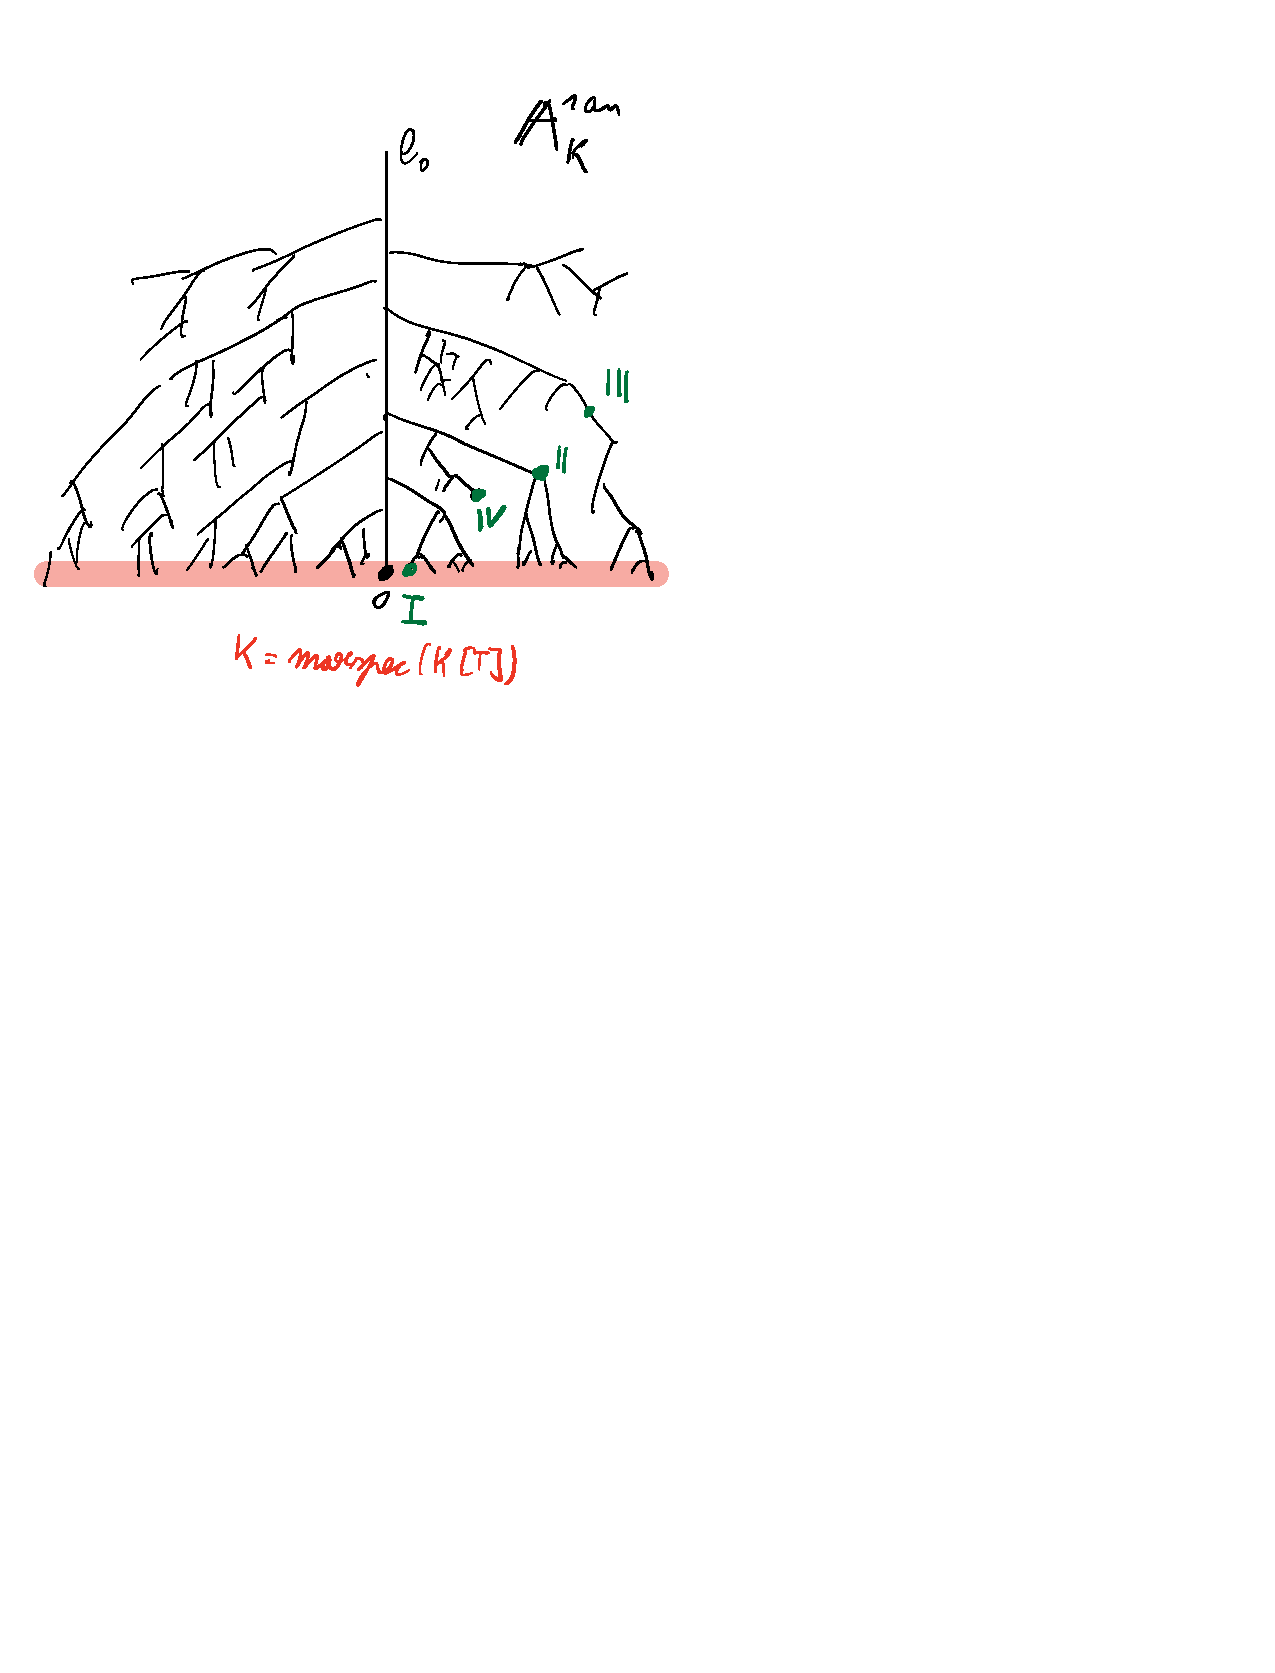
\includegraphics[width=0.5\textwidth]{figures/affine_line}
	\caption{The Berkovich affine line $\aff_K^{1, \text{an}} = \mathcal{M} (K[T])$, with the line $\ell_0$ from \cref{eq:line_in_A_1}}
	\label{fig:affine_line}
\end{figure}

There are other ways of recognizing type I, II, III and IV points, which will generalize better, when we look at Berkovich spectra of other curves. One is topological and the other one is purely algebraic. 

\begin{proposition}
	Let $x \in \aff_K^{1,\text{an}}$. 
	Let $C = \pi_0(\aff_K^{1, \an}\setminus \{ x\} )$ be the set of connected components of the punctured affine line. 
	\begin{itemize}
		\item If $x$ is of type I  or IV then $C$ has only one element.
		\item If $x$ is of type II then there a natural morphism $C \simeq k \cup \{\infty\} $. Recall that $k = \tilde K = K^{o} / K^{oo} $. 
			So $x$ is an branch point where infinitely many branches connect. 
		\item If $x = |\cdot |_{B(a, r)}$ is of type III then $|C| = 2$. One component consists of all disks contained in $B(a, r)$, (and type IV points corresponding to decreasing sequences of disks in $B(a,r)$) and the other one are all the leftover points. 
	\end{itemize}
\end{proposition}
\begin{figure}[h]
	\centering
	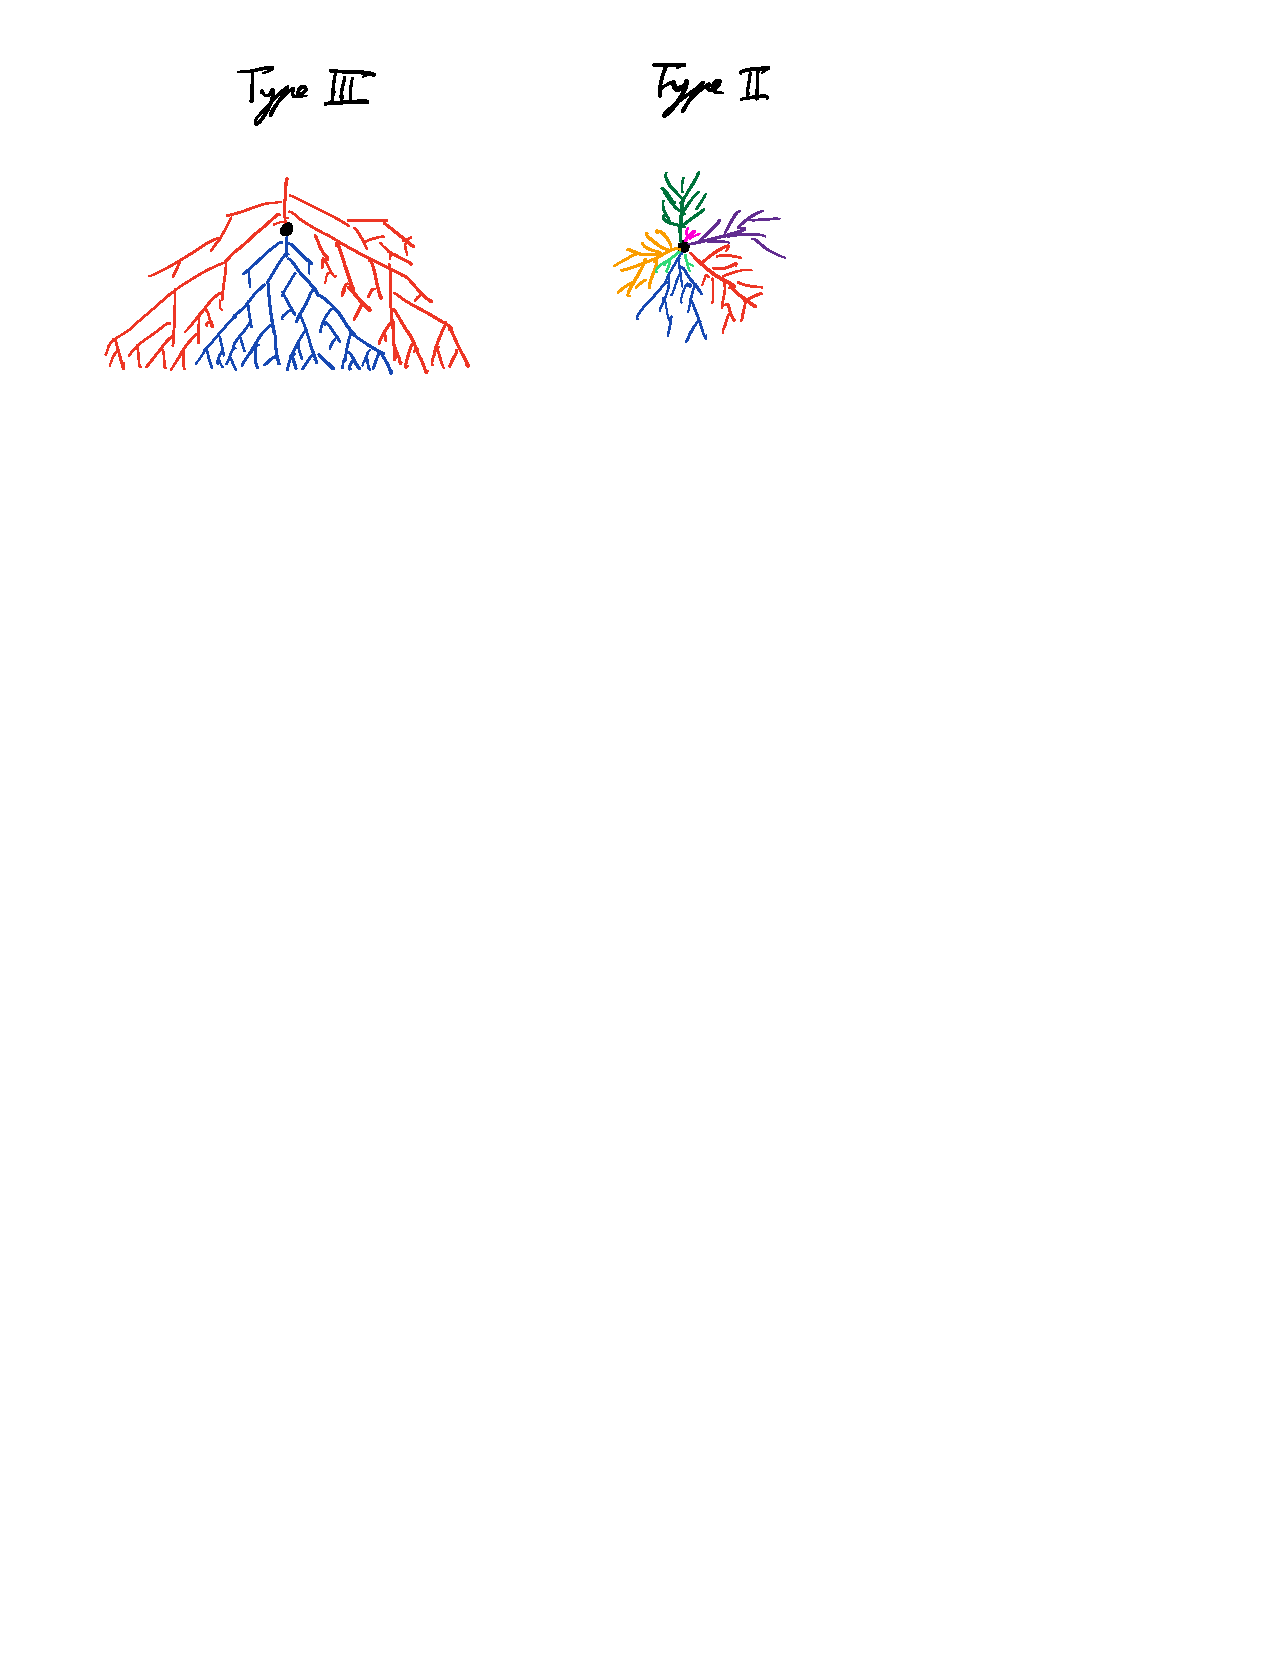
\includegraphics[width=0.7\textwidth]{figures/type2_type3.pdf}
	\caption{Recognizing type II and type III points by connected components/tangent directions}
	\label{fig:figures-type2_type3-pdf}
\end{figure}
The algebraic way to classify the points of $\aff_K^{1,\text{an}}$ is by using Abhyankar's inequality. 
\begin{definition}
	Let $K \subset L$ be a non-archimedean field extension. 
	Then we define \[
		E_{\frac{L}{ K}} = \dim \frac{|L^{\times }|}{|K^{\times }|} \otimes_\Z \Q, \qquad F_{L / K} = \trdeg(\tilde L / \tilde K)
	.\] 
\end{definition}

\begin{theorem}[Abhyankar's inequality]
	Let $K \subset H \subset L$ be non-archimedean rings extending each others norm. Assume that $L$ is algebraic over $\hat{H}$ and that $H$ is of transcendence degree $n$ over $K$. Then \[
	E_{L / K} + F_{L / K}  \le n
	.\] 
\end{theorem}

If $x \in \aff_K^{1, \text{an}}$ is a norm (not a seminorm) then its residue field $\mathcal{H} (x)$ is a completion on $K(T)$ with respect to the norm induced by $x$. As $K(T)$ is of transcendence degree 1 Abhyankar's inequality states that \[
	E_{\mathcal{H} (x) / K} + F_{\mathcal{H} (x) / K} \le 1
.\] 
This also allows us to classify points, because either both $E_{\mathcal{H} (x) / K}, F_{\mathcal{H} (x) / K}$ are zero, or exactly one is $1$. 
\begin{proposition}[2.3.3.3 in \cite{temkinIntroductionBerkovichAnalytic2010}]
	Let $x \in \aff_K^{1, \text{an}}$, then 
	\begin{itemize}
		\item $x$ is of type I if $\mathcal{H} (x) = K$
		\item $x$ is of type II if $F_{\mathcal{H} (x) / K} = 1$ and $E_{\mathcal{H} (x) / K} = 0$. 
		\item $x$ is of type III if $F_{\mathcal{H} (x) / K} = 0$ and $E_{\mathcal{H} (x) / K} = 1$.
		\item $x$ is of type IV if $\mathcal{H} (x) \subsetneq K$ and  $F_{\mathcal{H} (x) / K} = E_{\mathcal{H} (x) / K} = 0$.
	\end{itemize}
\end{proposition}

Type IV points are not rare. It might be counter intuitive that in a complete ring there exists a decreasing sequence of closed disks that has empty intersection. 
But in practice almost all fields have type  IV points. 
The trick is that the radii of these disks do not converge to $0$. 
\begin{example}[type IV point]\label{ex:type4point}
	Let $K = (\Q_p[\sqrt[2]{p} ,\sqrt[3]{p}, \sqrt[4]{p},\ldots])^{\wedge}  $ for some prime $p$. 
	Define 
	\begin{align*}
		a_n &= \sum_{i = 1}^{n} p^{-\frac{1}{n}}\\
		r_n &= p^{\frac{1}{n + 1}} \\
		B_n &= B(a_n, r_n) 
.\end{align*}
Then $|a_n - a_{n + 1}| = r_n$ and $r_{n + 1} \le r_n$ so the $B_{n + 1} \subset B_n$ and the sequence $(B_n)_n$ is decreasing. 
Now we have to show that the intersection $B = \bigcap_{i = 1} ^{\infty} B_n$ is non-empty. 

Let $x \in \C_p$. Then $x = \sum_{i = 0}^{m} b_i p^{c_i}$ where $m$ is either finite or $m = \infty, |b_i| = 1$ and $c_i$ is an increasing sequence such that $c_i \to \infty $. Suppose that  $x \in B$, then $x \in B_n$ for every $n$, and thus we see that  $b_i = p^{\frac{-1}{i}}$ for any $i = 1, \ldots, n$.  
This is true for any $n $, so in particular we find that $b_i = p^{-\frac{1}{i}}$ for any $i$ .
But this contradicts that $b_i$ is unbounded. 

Unfortunately the field in this example is non algebaicially closed. 
The algebraically closed field $\C_p$ also has type IV points, but the proof is a bit more subtle. See \cite[][sec. 3.4]{robertCoursePadicAnalysis2000}.
\todo{Make this more rigorous}
\end{example}
